% -*- root: root.tex -*-
\RequirePackage[l2tabu, orthodox]{nag}                  % Checks for obsolete syntax and package % Layout
\documentclass[11pt,a4paper,oneside]{article}

%% font
\usepackage{MnSymbol}
\usepackage[mathlf,textlf]{MinionPro}
\usepackage[T1]{fontenc}
\usepackage{enumitem}
\usepackage[utf8]{inputenc}

%% Author
\def\myaffiliation{University of Copenhagen}
\def\myauthor{Rud Faden}
\def\myemail{rud.faden@econ.ku.dk}
\def\mytitle{No cure no pay contracts with limited liability}
\def\mykeywords{Information aggregation, physician,}

%% packages
\usepackage[drafting]{faden}
\pgfplotsset{compat=1.9}
\usetikzlibrary{decorations.pathreplacing}
\graphicspath{{../fig/}}
\usepackage{commath}
\usepackage[colorinlistoftodos,draft]{todonotes}        % todo notes
\setlength{\marginparwidth}{3.5cm} % fix for todo notes


%% custom macroes 

%% biblatex path
\addbibresource{Remote.bib}

% Author and title
\title{\mytitle}
\author{
{\myauthor} \\
\textit{\small \myaffiliation} \\
\small{\texttt{\href{\myemail}{\myemail}}}
}
\date{\today} % no date

%% Version control
\immediate\write18{sh ./vc}
%%% This file has been generated by the vc bundle for TeX.
%%% Do not edit this file!
%%%
%%% Define Git specific macros.
\gdef\GITHash{9d5e3b469d5f4d8f56c54cfc33fcab676c8905ff}%
\gdef\GITAbrHash{9d5e3b4}%
\gdef\GITParentHashes{904e5d3ddc0482da848ff729ca2451b0fd5c4aee}%
\gdef\GITAbrParentHashes{904e5d3}%
\gdef\GITAuthorName{Rud Faden}%
\gdef\GITAuthorEmail{rudfaden@gmail.com}%
\gdef\GITAuthorDate{2015-04-27 11:47:18 +0200}%
\gdef\GITCommitterName{Rud Faden}%
\gdef\GITCommitterEmail{rudfaden@gmail.com}%
\gdef\GITCommitterDate{2015-04-27 11:47:18 +0200}%
%%% Define generic version control macros.
\gdef\VCRevision{\GITAbrHash}%
\gdef\VCAuthor{\GITAuthorName}%
\gdef\VCDateRAW{2015-04-27}%
\gdef\VCDateISO{2015-04-27}%
\gdef\VCDateTEX{2015/04/27}%
\gdef\VCTime{11:47:18 +0200}%
\gdef\VCModifiedText{\textcolor{red}{with local modifications!}}%
%%% Assume clean working copy.
\gdef\VCModified{0}%
\gdef\VCRevisionMod{\VCRevision}%



\begin{document}
\maketitle
\begin{abstract}
This paper examines a principal agent model in which a risk neutral physician makes an ex-ante effort choice while receiving payment from a risk neutral
principal. It is assumed that the physician is subject to limited liability, such
that he cannot be punished for bad outcome, but only rewarded for good outcomes.
\VCModified
\end{abstract}

\section{Introduction} % (fold)
\label{sec:introduction}
In the last couple of decades there has been an increasing interest in constructing payment schemes that increase hospital output. Most attention seems to be on reimbursing hospitals based on activity via casemix based payment schemes. Little attention has been given to the physicians incentives. Maybe because fixed hours and wages are the norm for most hospital employed physicians. This is quite surprising as fixed wages are known to give no production incentive when effort is unobservable. \todo{Insert source} I.e.\ the physician chooses the lowest possible level of effort. This effort level might be limited by some ethical constraint or by fear of malpractice lawsuits. This fact is even more surprising when comparing to other medical fields, like family medicine, where incentive contracting has been applied for a number of years. 

Incentive contracts are, nevertheless, very conservative in health care. Focus seems to be on constructing per item fees that increase physician productivity, without lowering quality. Such payment schemes totally ignore where on the production schedule and thereby also the incentive in creating payment mechanisms that only reward the physician for after some target goal, with respect to quality and quantity has been meet. 

For example, one might imagine that in fertility treatment, the physician will only get paid when the patients has been successfully treated or a surgeon only paid when an operation is a success. Such contracts, usually known as contingent fee contract, are well known in other industries. A typical example, is real estate agents, which are only paid in the case the house is actually sold, a the fee system for lawyers in the US, where the plaintiff only pays a fee if the case is won. However, in may of those cases, the agents takes a loss if outcome is not successful. In the light of this \textcite{Lambert2005No} analyzed the physician problem in a two state case, and found that the agent should pay a penalty to the principal if the bad state occurs. But in many environments, like a hospital, such contracts would probably be very unpopular and a practical implementation impossible. A more feasible solution is to let the physician be bounded by limited liability, such that he is only rewarded for good outcomes and not punished for bad outcomes. Similarly I also implement that the hospital should not be forced to pay more than the value of the production.  

In this paper, I therefore develop a model, based on \textcite{Innes1990Limited}, where a hospital (the principal) wishes to maximize output, which could be DRG payments or some other monetary measure of productivity. In doing so, the hospital employs a physician (the agent). But physicians effort is uncontractible. Moreover the contract is bounded below, by the physician limited liability and above by the value of the production. 
% section introduction (end)
\section{Model} % (fold)
\label{sec:model}
There is a risk neutral physician that cures a continuum of patients with a value to the principal of $y\in[0,\infty)$ and receives payment $R(y)$. The physician cures patient with effort $e$. I assume that the probability of curing a patient is monotonically increasing in effort (monotone likelihood ratio property), such that 
\begin{align}
    \pder{y}\left(\frac{g_e(y\mid e)}{g(y\mid e)}\right)>0 \label{eq:mlrp}
\end{align}
for all $e>0$ and $y\ge 0$. In addition I assume that $E[y|e=0]=0$. Further I also assume that the distribution functions satisfies convexity of the distribution function (CDFC).\footnote{The CDFC assumption implies that $\pder[G(y|e)][2]{e}\geq0$. See \textcite[][p. 1362]{Rogerson1985FirstOrder}}

The principal observes the physicians value of cured patients ex-ante. Therefore the hospital specifies a contract that pays the physician $R(y)$.

Further it is assumed that the payoff is bounded by limited liability. This implies that (i) the principal cannot be required to pay the physician more than the value of the production, and (ii) the physician cannot be required to make payments to the hospital.  Therefore the payment function is bounded by $0\leq R(y)\leq y$.

Let $U(R,e)$ denote the physicians separable, continuous and twice differential utility function given by 

\begin{align}
    U(R,e)=\int_0^\infty u(R(y))g(y|e)\dif y-C(e) \label{eq:utility}
\end{align}

and the hospitals payoff is given by 
\begin{align}
    V(y,R(y))=\int_0^\infty (y-R(y))g(y|e)\dif y
\end{align}
and the hospital requires a minimum production of $y_L^0$ to participate. 
Unfortunately neither existence or uniqueness of a solution to \cref{eq:utility} can be guaranteed. To reduce the ambiguity I introduce the following assumptions. 
\begin{assumption}
\label{asump:unique-solution}
The agent utility is increasing and concave in $R$ and decreasing and convex in $C(e)$. Further, $\pder[][2]{e}U(R,e)<0$ for all $e$, and therefore, there is a unique solution to the physicians effort choice problem.
\end{assumption}

%section model (end)
\section{Fixed wage} % (fold)
\label{sec:fixed_wage}
When effort is observable the first best contract is the solution to 
\begin{subequations}
\label{eq:khun-tucker-fw}
\begin{align}
    \max_{R,e} & \int_0^{\infty}u(R(y))g(y|e)\dif y-C(e) \\
    \text{s.t. }    & \int_{0}^{\infty} (y-R(y))g(y|e)\dif y\geq y_L^0
\end{align}
\end{subequations}
for all $R\in[0,y]$ is given by 
\[
    \frac{1}{u'(R(y))}=\frac{1}{\lambda}
\]
I.e.\ the lowest fixed wage, that fulfills the hospitals participation constraint. This is the \emph{first-best} solution to the optimization problem. 

However, when effort is not contractible, a fixed wage will induce the physician to choose the lowest level of effort that clears the hospitals participation constraint. This will happen only if $U(1/\lambda,e)\geq U(y,0)$. Let the effort level  $\underline{e}$ that solves $E[y|e]=y^0_L$, which is lager than $0$, given that $E[y|e=0]=0$. Let $\underline{y}$ be the level of production, when effort is $\underline{e}$. The hospitals profit is then 
\[
 \underline{y}-\frac{1}{\lambda}
\]
and the physicians utility is 
\[
 u\left(1\big/\lambda\right)-C(\underline{e})
\]
This solution is clearly suboptimal, as long as there exists another contract $R(y)$ for which it holds that $u(R(y))\geq C(e)$.

% section fixed_wage (end)
\section{Optimal payment with a risk neutral agent} % (fold)
\label{sec:optimal_payment_with_a_risk_neutral_agent}




Given \cref{eq:utility} and a fixed payment function $R(y)$, the physician will choose effort to solve the following problem
\begin{subequations}
\label{eq:khun-tucker}
\begin{align}
    \max_{R,e} & \int_0^{\infty}R(y)g(y|e)\dif y-C(e)\label{subeq:khun-tucker1} \\
    \text{s.t. }    & \int_{0}^{\infty} (y-R(y))g(y|e)\dif y\geq y_L^0 \label{subeq:khun-tucker2} \\
                    & E[u(R,e)|e]\leq E[u(R,e^*)|e] \label{subeq:khun-tucker3}\\
                    & 0\leq R(y)\leq y \label{subeq:khun-tucker4}
\end{align}
\end{subequations}
To find a solution to \cref{eq:khun-tucker} is difficult and few general results can obtained. To make the problem more tractable incentive comparability constraint in \cref{subeq:khun-tucker3} is often replaced by the first order derivative. 

\begin{proposition}
\label{prop:payment-function}
If $R$ solves the maximization problem in \cref{subeq:khun-tucker1}, then there is some threshold value $y^*$, such that 

\[
    R^*(y)=\begin{cases}
                0 & \text{for } y< y^* \\
                y & \text{for } y\geq y^*
            \end{cases}            
\]
\end{proposition}

\begin{proof}
Replacing \cref{subeq:khun-tucker3} with it's  first order condition, and writing down the Lagrangian I get that 
\begin{align}
    \mathcal{L}=R(y)g(y|e)-C(e)+\mu [R(y)g_e(y|e)-C_e(e)]+\lambda [(y-R(y))g(y|e)-y_L^0]
\end{align}
which can also be written as 
\begin{equation}
\begin{split}
   R(y)\left[g(y|e)+\mu g_(y|e)\right]+(y-R(y))\lambda &g(y|e)+ \\
                         & yg(y|e)-\mu C_e(e)-\lambda y_L^0 \label{eq:lagrange}
\end{split}
\end{equation}

Only the first to terms of \cref{eq:lagrange} depends on the size of $R(y)$ and thereby determines the maximum. If the first term is larger than the second term

\begin{align}
     R(y)\left[g(y|e)+\mu g_(y|e)\right]>(y-R(y))\lambda g(y|e) \label{eq:max-payment}
\end{align}

the whole expression is increasing in $R(y)$, therefore $R(y)$ should be set to it's maximum $R(y)=y$. If the opposite is true 
\begin{align}
     R(y)\left[g(y|e)+\mu g_(y|e)\right]<(y-R(y))\lambda g(y|e) \label{eq:min-payment}
\end{align}
the expression is decreasing in $R$, and $R(y)$ should be set to it's minimum $R(y)=0$. Note that \cref{eq:min-payment} can be written as

\begin{align}
   1+\mu \frac{g_e(y|e)}{g(y|e)}<\lambda \label{eq:min-payment-2}
\end{align}

Given \cref{eq:mlrp}, the left hand side of \cref{eq:min-payment-2} is increasing in $y$ this inequality is satisfied for some $y$ below a threshold level $y^*$. Above $y^*$ \cref{eq:max-payment} holds. Thereby the payment function is 0 for some $y<y^*$ and $y$ for some level above $y> y^*$ as stated in \cref{prop:payment-function}.

What remains is to show that the solution to \cref{eq:khun-tucker} is in fact an optimum. Following \textcite{Rogerson1985FirstOrder} it is sufficient to show that $\mu>0$. If $\mu\leq0$, payment is non-increasing in output. By \cref{asump:unique-solution} the physician therefore chooses $e=0$. However, $e=0$ is not feasible because of the assumption that $E[y|e=0]=0$ and condition \cref{subeq:khun-tucker2}. Therefore for $e>0$, $\mu$ must be positive. 
\end{proof}

\begin{figure}[htbp]
    \centering
    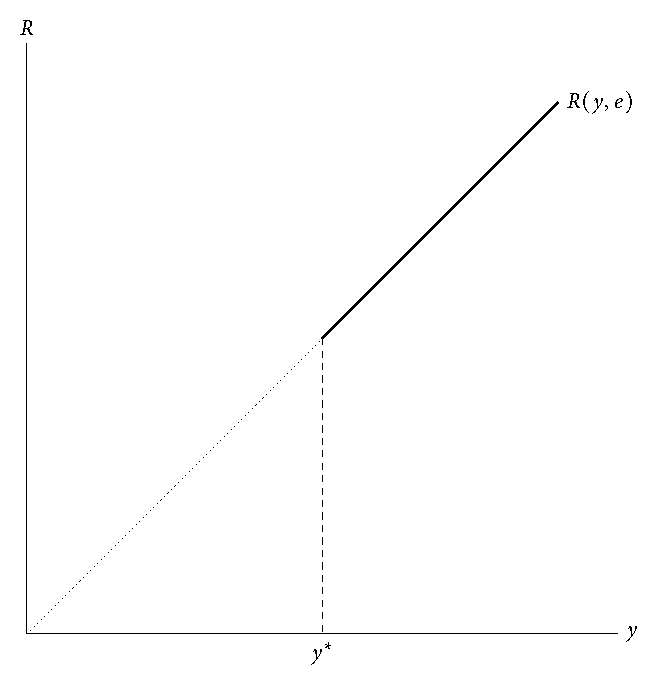
\includegraphics[width=0.95\textwidth]{optimal-R.pdf}
    \caption{The payment function $R(y)$. Before $y^*$ the physician is payed nothing and after $y^*$ the physician is the payed maximum of $R(y)$ }
    \label{fig:label}
\end{figure}

\subsection{An alternative proof} % (fold)
\label{sub:an_alternative_proof}
Give \cref{eq:khun-tucker}  Lagrangian is
\begin{align}
    \begin{split}
        \mathcal{L}=R(y)g(y|e)-C(e)+\mu [R(y)g_e(y|e)-C_e(e)]+ \\ 
        \lambda [(y-R(y))g(y|e)-y_L^0]+\theta(y) R(y)+\theta(y)\left(y-R(y)\right)
    \end{split}
\end{align}
The first order conditions are
\begin{subequations}
\label{eq:foc}
\begin{align}
    g(y|e)\left[1-\lambda+\mu \frac{g_e(y|e)}{g(y|e)}\right]+\theta(y)-\eta(y) \label{eq:foc1} \\
    R(y)\left[(1-\lambda)g_e(y|e)+\mu g_{ee}(y|e)\right]-C_e(e)-C_{ee}(e)
\end{align}
\end{subequations}
Because of non-negativity and complementary slackness conditions for $\theta(y)$ and $\eta(y)$, \cref{eq:foc1} yields
\begin{subequations}
\label{eq:KT-analysis}
\begin{alignat}{3}
\phi(y,e) = g(y|e)\left[1-\lambda+\mu \frac{g_e(y|e)}{g(y|e)}\right]
   & \: > \: & 0 &\enspace \Rightarrow &&\enspace R(y)=y \label{subeq:large-y}\\
 \phi(y,e)   & \: = \: & 0 &\enspace \Rightarrow &&\enspace R(y)\in [0,y] \label{subeq:interval-y} \\
 \phi(y,e)   & \: < \: & 0 &\enspace \Rightarrow &&\enspace R(y) =0 \label{subeq:small-y}
\end{alignat}
\end{subequations}

It is clear from \cref{eq:foc1,eq:mlrp} that for $y$ large enough \cref{subeq:large-y} is always feasible. However, feasibility of \cref{subeq:interval-y,subeq:large-y} is not guaranteed, even for $y=0$ However, if $1>-\lambda+\mu \frac{g_e(y|e)}{g(y|e)}$, which is likely, then there must be some range of $e$ where \cref{subeq:large-y} (and thereby also \cref{subeq:interval-y}) holds. 

% subsection an_alternative_proof (end)
% section optimal_payment_with_a_risk_neutral_agent (end)
\section{Optimal payment with a risk averse agent} % (fold)
\label{sec:optimal_payment_with_a_risk_averse_agent}
I know introduce a risk averse agent with utility $u(R(y))$, such that $u'>0$ and $u''<0$. The problem is then restated as 

\begin{subequations}
\label{eq:khun-tucker-ra}
\begin{align}
    \max_{R,e} & \int_0^{\infty}u(R(y))g(y|e)\dif y-C(e)\label{subeq:khun-tucker-ra1} \\
    \text{s.t. }    & \int_{0}^{\infty} (y-R(y))g(y|e)\dif y\geq y_L^0 \label{subeq:khun-tucker-ra2} \\
                    & E[u(R,e)|e]\leq E[u(R,e^*)|e] \label{subeq:khun-tucker-ra3}\\
                    & 0\leq R(y)\leq y \label{subeq:khun-tucker-ra4}
\end{align}
\end{subequations}

Using the first order approach as before I get that 

\begin{subequations}
\label{eq:lagrange-ra}
\begin{align}
    u'(R(y))g(y|e)\left[1-\lambda+\mu \frac{g_e(y|e)}{g(y|e)}\right] + \theta(y)-\eta(y)=0 \\
    g_e(y|e)\left[(1+\mu)u(R(y))\frac{g_{ee}(y|e)}{g_e(y|e)}+\lambda(y-R(y))\right]-c_e(e)-c_{ee}(e)
\end{align}
\end{subequations}

Again define 
\[
    \phi(y,e) = u'(R(y))g(y|e)\left[1-\lambda+\mu \frac{g_e(y|e)}{g(y|e)}\right]  + \theta(y)-\eta(y)
\]

\begin{subequations}
\label{eq:KT-analysis-ra}
\begin{alignat}{3}
    \phi(y,e) & \: > \: & 0 & \enspace \Rightarrow & & \enspace R(y)=y \label{subeq:large-y-ra}\\
    \phi(y,e) & \: = \: & 0 & \enspace \Rightarrow & & \enspace R(y)\in [0,y] \label{subeq:interval-y-ra} \\
    \phi(y,e) & \: < \: & 0 & \enspace \Rightarrow & & \enspace R(y) =0 \label{subeq:small-y-ra}
\end{alignat}
\end{subequations}

Further, by implicitly defining $R(y)\in[0,y]$ by 
\[
    \frac{1}{u'(R(y))}=\frac{1}{\lambda}+\frac{\mu}{\lambda}\frac{g_e(y|e)}{g(y|e)}
\]
and noting that by concavity of $u(R(y))$, $R(y)$ is increasing in $e$. However, when the physician is risk neutral, the physicians utility is linear in $y$. Therefore he will apply effort in a constant rate as $y$ increases. When the agent is risk averse, he requires an increasing amount of payment to apply the same increase in effort. Therefore the effort he provides is decreasing in $R(y)$. \todo{Det var det jeg skrev om tidligere}


\begin{proposition}
A risk averse physician will apply weakly less effort than a risk neutral physician. \todo[color=red]{This should be refined and proofed}
\end{proposition}
%section optimal_payment_with_a_risk_averse_agent (end)
\printbibliography%
\listoftodos
\end{document}